\input{../common}
\everymath{\displaystyle}
\begin{document}
  %<*content>
  \lesson{algebra}{9}{Variables aléatoires}
  
  \begin{lemma}
 On lance deux fois de suite une pièce de monnaie  et on note  les côtés apparus :  Pile ( $ P$ ) ou Face ($F $).\\L'ensemble des issues est:\\ $ \Omega=\accol{(P,P);(F,F);(F,P);(P,F)} $.\\ On convient du jeu suivant: on  gagne $ 5F $  chaque fois que sort Pile et on perd $ 2F $ chaque fois sort Face. \\ Par exemple à l'issue $ (F,P) $ on perd 2F et gagne 5F donc le gain résultant est $ -2+5=3 $F.
 \begin{enumerate}
\item On note par  G un gain  possible pour un joueur. Donner toutes les valeurs $ x $ de G.
\item Justifier que G est une application et préciser  son ensemble de départ et d'arrivée.
\item Pour chacune des valeurs  $ x $  de G, calculer la probabilité de gagner $ x $ francs ?\\ On  notera cette probabilité par $P(G  =x)$.
\item Vérifier que la somme des probabilités trouvées est égale à 1.
\end{enumerate}

  \end{lemma}
\begin{definition}
$ \Omega $  est l'ensemble des issues d'une expérience aléatoire.\\ Une \textbf{variable aléatoire } sur  $ \Omega $  est une fonction qui, à chaque issue de $ \Omega $ , associe un nombre réel.
\end{definition}
 \begin{notation}
 Une variable aléatoire  est généralement notée $X $, $ Y $ ,$Z $ $ \cdots $\\ Lorsque $ x $ désigne un nombre réel, dire << $ X $ prend la valeur $ x $>>  est un événement, il est noté $ (X=x) $.\\$ (X< x) $ désigne l'événement << $ X $ prend une  valeur strictement inférieure à $ x $>> \\
  $ (X\geq x) $ désigne l'événement << $ X $ prend  au moins une fois la  valeur  $ x $>> , c'est le contraire  de l'événement précédent. 
  
   \end{notation}
   \begin{example}
   On reprend l'exercice de l'activité.\\
On lance deux fois de suite une pièce de monnaie  et on note  les côtés apparus : $ P$ ou $F $.\\L'ensemble des issues est:\\ $ \Omega=\accol{(P,P);(F,F);(F,P);(P,F)} $.\\ On gagne $ 5F $  chaque fois que sort Pile et on perd $ 2F $ chaque fois sort Face. On définit ainsi une variable aléatoire $X $ sur $ \Omega $  qui prend les valeurs ; $-4 $; \;$  3$   et $ 10$.\\L'événement $ (X=3) $ est réalisé par  les issues $ (F,P)$ et $(P,F) $
   \end{example}
   \subsection{Loi de probabilité d'une variable aléatoire}
\begin{definition}
Une loi de probabilité est définie sur un ensemble $ \Omega $  d'issues.\\ $ X $  est une variable aléatoire  définie sur $ \Omega $ et $ E=\accol{x_{1},x_{2},\cdots, x_{n}} $ est l'ensemble des valeurs prises par $ X. $\\Lorsqu'on associe  à chaque valeur  $ x_{i} $ , la probabilité de l'événement  $ (X=x_{i}) $, on définit une loi de probabilité sur $ E. $\\ Cette loi est appelée \textbf{loi de probabilité de variable aléatoire $ X $.}
\end{definition}

\begin{remark}
 On présente souvent la loi de probabilité d'une variable aléatoire  discrète $ X $ à l'aide d'un tableau.

\begin{tabularx}{\textwidth}{|X|X|X|X|X|}
\hline
Valeurs de $ X$ &$ x_{1}$& $x_{2}$ &$\cdots$  &$x_{n}$\\
\hline
$ P(X=x_{i}) $ & $ p_{1} $& $ p_{2} $  &$\cdots  $ & $ p_{n} $\\
\hline
\end{tabularx}

On a: $ P(X=x_{1})+P(X=x_{2})+\cdots +P(X=x_{n})= p_{1}+p_{2}+\cdots + p_{n}=\displaystyle\sum_{k=1}^n p_{k}= 1 $
\end{remark}
\begin{example}
On reprend l'exemple de l'activité d'introduction.

 La probabilité de l'événement  $ (X= -4) $  est la probabilité de l'issue $ (F,F) $ c'est-à-dire $ P(X=-4) =\frac{1}{4}$\\
La probabilité de l'événement  $ (X= 3) $  est la somme des  probabilités des issues $ (P,F) $  et  $ (F,P) $ c'est-à-dire $ P(X=3) =\frac{1}{4}+\frac{1}{4}=\frac{1}{2}$.\\
La probabilité de l'événement  $ (X= 10) $  est la probabilité de l'issue $ (P,P) $ c'est-à-dire $ P(X=10) =\frac{1}{4}$\\ La loi de la variable aléatoire $ X $ est résumée dans le tableau ci-dessous.\\

\begin{tabularx}{\textwidth}{|X|X|X|X|X|}
\hline
 $ x_{i}$ & $ -4$ & $ 3$ & $10 $\\
\hline
$ P(X=x_{i}) $ & $ \frac{1}{4} $& $ \frac{1}{2} $   & $ \frac{1}{4} $\\
\hline
\end{tabularx}
\end{example}
\subsection{Fonction de répartition}
\begin{definition}
Soit $ X $  une variable aléatoire définie sur un univers $ \Omega $ muni d'une probabilité P.\\
La fonction de répartition de $ X $  est l'application $ F $ de $ \Rr $ vers $ \intff{0}{1} $ définie par:\;$ F(x)=P (X\leq x) $
\end{definition}

\begin{example}
Reprenons l'exemple  de l'activité.\\
$ F $ est définie par: $\sysq{F(x)=0,\;\; \text{si}\;\; x< -4}{F(x)=\frac{1}{4}, \;\; \text{si}\;\; -4\leq x< 3}{F(x)=\frac{3}{4}, \;\; \text{si}\;\; 3\leq x< 10}{F(x)=1, \;\; \text{si}\;\; 10\leq x} $

\bigskip

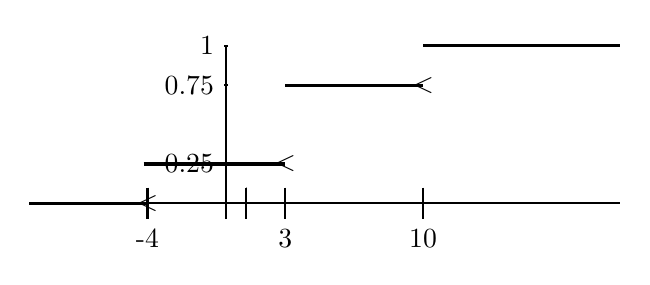
\begin{tikzpicture}[xscale= 0.25,yscale=2]
%\draw[very thin,style=gray!60,step=0.1] (-7,-4) grid (9,9);
\draw[very thin] (-10,-0.1)  (20,1);
\draw[thick] (-10,0) -- (20,0);
\draw[thick] (0,-0.1) -- (0,1);
\foreach\x in {-4,,,,,,,3,,,,,,10}
{
\draw[thick] (\x,0.1) -- (\x,-0.1) node[below] {\x};
}
\foreach\y in { 0.25,0.75,1 }
{
\draw[thick] (0.1,\y) -- (-0.1,\y) node[left] {\y};
}
\draw[very thick,domain= -10:-4]  plot(\x,0);
\draw[ very thick,domain= -4.2:3]  plot(\x,0.25);
\draw [very thick, domain= 3:10]  plot(\x,3*0.25);
\draw[very thick, domain= 10:20]  plot(\x, 1);
%\draw[domain= -5:1.5]   plot(\x,-2*\x-1);
\node at (-4,0) {$ < $};
\node at (10,0.75) {$ < $};
\node at (3,0.25) {$ < $};
\end{tikzpicture}

\end{example}
\begin{remark}
\begin{itemize}
\item  $ F $ est une fonction croissante en escalier. 
\item  La  représentation graphique de F correspond en statistiques à la courbe des fréquences cumulées croissantes.
\end{itemize}
\end{remark}

\subsection{Paramètres d'une variable aléatoire}
\textbf{Espérance, variance et écart-type}
 \begin{definition}
 Une loi de probabilité est définie sur un ensemble $ \Omega $  d'issues.\\ $ X $  est une variable aléatoire  définie sur $ \Omega $ dont la loi de probabilité est résumée dans le tableau ci-dessous.
\bigskip

\begin{tabularx}{\textwidth}{|X|X|X|X|X|}
\hline
Valeurs de $ X$ &$ x_{1}$& $x_{2}$ &$\cdots$  &$x_{n}$\\
\hline
$ P(X=x_{i}) $ & $ p_{1} $& $ p_{2} $  &$\cdots  $ & $ p_{n} $\\
\hline
\end{tabularx}


\begin{itemize}
\item L'espérance de la variable aléatoire $ X $  est le nombre réel, noté E$ (X) $  défini par :
  \[ \text{E}(X)=p_{1}x_{1} + p_{2}x_{2} +\cdots + p_{n}x_{n} =\displaystyle \sum_{k=1}^n p_{k}x_{k} \]
  
   \item  La variance  de la variable aléatoire $ X $  est le nombre réel  positif , noté V$ (X) $  défini par :
  \[ \text{V}(X)=p_{1}\paren{x_{1}-\text{E}(X)}^{2} + p_{2}\paren{x_{2}-\text{E}(X)}^{2} +\cdots + p_{n}\paren{x_{n}-\text{E}(X)}^{2} =\displaystyle\sum_{k=1}^n p_{k}\paren{x_{k}-\text{E}(X)}^{2}\]
\item L'écart-type  de la variable aléatoire $ X $  est le nombre réel  positif , noté $ \sigma(X) $  défini par :$$ \sigma(X)=\sqrt{\text{V}(X)}.$$
 \end{itemize}
\end{definition}

\begin{example}
On reprend l'exemple de la variable aléatoire $ X $ précédent.\\ $\text{E}(X)=\frac{1}{4}(-4)+\frac{1}{2}\times 3 +\frac{1}{4}\times 10 =3$ francs.\quad $ \text{E}(X)=3$ francs    signifie qu'en jouant un grand  nombre de fois  à ce jeu , un joueur peut espérer gagner $ 3$ francs    en moyenne.\\ $ \text{V}(X)= \dfrac{1}{4}(-4-3)^{2}+\dfrac{1}{2}(3-3)^{2}+\dfrac{1}{4}(10-3)^{2}=\dfrac{49}{2} $ \;\;et \quad $ \sigma(X)=\dfrac{7\sqrt{2}}{2} $.
\end{example}
\begin{remark}
\begin{itemize}
\item   L'espérance mathématique correspond, en statistiques, à la moyenne.
\item L'espérance et l'écart-type sont exprimés dans la même unité que les valeurs $ x_{i} $ prises par $ X $
\item Un jeu est dit équitable lorsque $ \text{E}(X)=0.$
\end{itemize}
\end{remark}
\begin{property}
Soit $ X  $ une  variable aléatoire. On a \; $ \text{V}(X)=  \text{E}(X^{2})- (\text{E}(X))^{2} $
\end{property}
\textbf{Démonstration}\\
On a V(X)$ =\displaystyle\sum_{k=1}^n p_{k}\paren{x_{k}-\text{E}(X)}^{2}=\displaystyle\sum_{k=1}^n p_{k}x_{k}^{2}-2\text{E}(X)\displaystyle\sum_{k=1}^n p_{k}x_{k}+ \paren{\text{E}(X)}^{2}\displaystyle\sum_{k=1}^n p_{k}$\\
Or $\displaystyle \sum_{k=1}^n p_{k}x_{k}=\text{E}(X) $,\;  $\displaystyle\sum_{k=1}^n p_{k}=1  $\; et  $\;\displaystyle \sum_{k=1}^n p_{k}x_{k}^{2}=\text{E}(X^{2}) $\\

V(X)$ =\text{E}(X^{2})-2\times \text{E}(X)\times \text{E}(X)+\paren{\text{E}(X)}^{2} =\text{E}(X^{2})- (\text{E}(X))^{2}$

\begin{property}[Admise]
$ X $  est une  variable aléatoire. Pour  tous nombres réels $a $ et $b $.
 $$\text{E}(aX+b)=a\text{E}(X)+b     \qquad  \text{et} \quad  \text{V}(aX+b)=a^{2}\text{V}(X) $$
\end{property}

   
  %</content>
\end{document}
